\documentclass{standalone}

\usepackage{pgfplots}
\usepackage{tikz}
\usetikzlibrary{positioning}
\usetikzlibrary{decorations.text}
\usetikzlibrary{decorations.pathmorphing}

\begin{document}
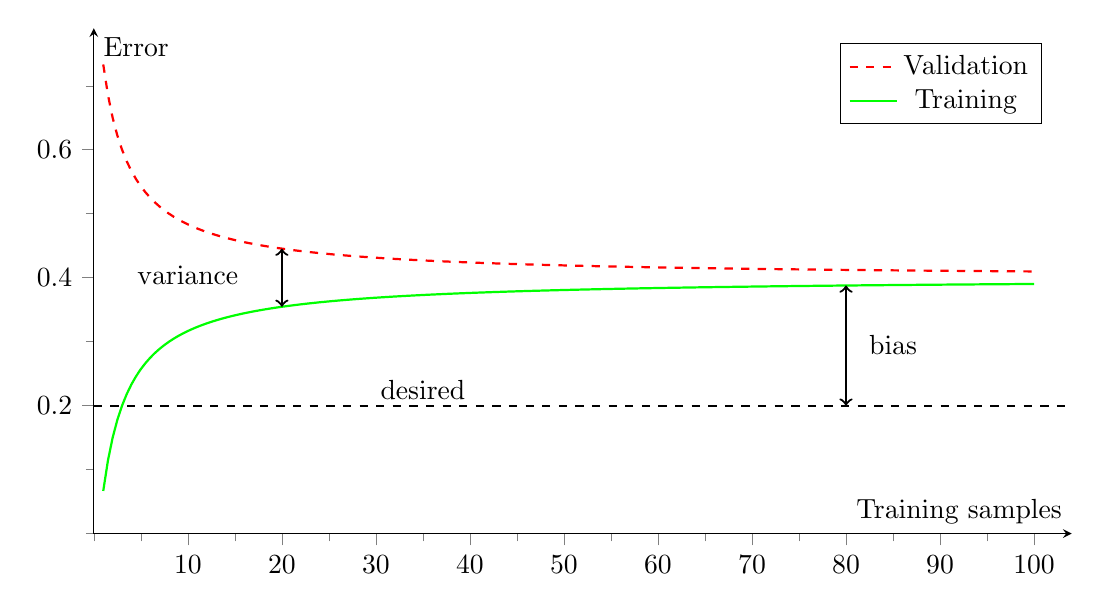
\begin{tikzpicture}
    \begin{axis}[
        legend pos=north east,
        axis x line=middle,
        axis y line=middle,
        grid = major,
        width=14cm,
        height=8cm,
        grid style={dashed, white}, % gray!30
        xmin=0,       % start the diagram at this x-coordinate
        xmax= 104,    % end   the diagram at this x-coordinate
        ymin= 0,      % start the diagram at this y-coordinate
        ymax= 0.79,   % end   the diagram at this y-coordinate
        axis background/.style={fill=white},
        xlabel=Training samples,
        ylabel=Error,
        tick align=outside,
        minor tick num=-3,
        tension=0.08]
      \addplot[domain=1:100, red, thick,samples=200,dashed] {1/(x+2)+0.4};
      \addplot[domain=1:100, green, thick,samples=200] {0.4-(1/(x+2))};

      % \draw[dashed,thick] (axis cs:0,0.4) -- (axis cs:110,0.4);
      \draw[dashed,thick] (axis cs:0,0.2) -- (axis cs:110,0.2);
      \draw[thick,<->] (axis cs:80,0.2) -- (axis cs:80,0.3878);
      \draw[thick,<->] (axis cs:20,0.3545) -- (axis cs:20,0.4454);
      \draw[decoration={text along path, text={desired}, text align={center}}, decorate] (axis cs:20,0.21) -- (axis cs:50,0.21);
      \draw[decoration={text along path, text={bias}, text align={center}}, decorate] (axis cs:80,0.28) -- (axis cs:90,0.28);
      \draw[decoration={text along path, text={variance}, text align={center}}, decorate] (axis cs:0,0.39) -- (axis cs:20,0.39);

      \addlegendentry{Validation}
      \addlegendentry{Training}
    \end{axis}
\end{tikzpicture}
\end{document}
